
\chapter{Genetické programování}

\section{Základní princip}
Genetické programování je evoluční technika, která vytváří počítačové programy. Cílem genetického programování je vyřešit co nejlépe zadaný problém.
Nespecifikujeme jak je potřeba ho vyřešit, ale víme, co je potřeba vyřešit.
\par
Každý program budeme nazývat jedincem a množině jedinců budeme říkat populace. Algoritmus pak běží iterativně v generacích. 
V každé iteraci se provede výběr nějakých jedinců z populace, ti se pomocí genetických operátorů upraví a nakonec se rozhoduje, kteří z nich přežijí do další generace.
Populaci na začátku iterace nazýváme rodiče a populaci, která bylo nakonci iterace pro další generaci, nazýváme potomky.
Každý program představuje jedno řešení daného problému. Kvalitu tohoto řešení ohodnocujeme takzvanou fitness funkcí. Čím vyšší hodnotu této funkce jedinec získá, tím lépe řeší daný problém.
\subsection{Reprezentace}

Program je obvykle reprezentovaný syntaktickým stromem. Stromy ve vnitřních uzlech obsahují funkce (neterminály) a v listech terminály.
Vyhodnocení stromu probíhá od listů ke kořeni a výsledek programu je pak hodnota kořenu.

\subsection{Inicializace populace}
Na začátku evoluce potřebujeme inicializovat populaci. Na počátku jsou jedinci vytvořeni náhodně. Obvykle se k vytvoření jedinců používají dvě metody.
První z nich je vytváření jedinců s pevně danou hloubkou stromu, kde v listech jsou vždy už jen terminály. Druhou metodou je stavět strom náhodně z předem daného počtu neterminálů.
Po vyčerpání počtu neterminálů se již opět přidají terminály jako listy. Tato metoda vytváří jedince různých velikostí a tvarů.
Častou praxí je prvotní populaci vytvořit tak, že každá z metod vytvoří polovinu jedinců. 

\subsection{Selekce}
V každé iteraci chceme vybrat několik jedinců, nad kterými budeme provádět různé genetické operátory. Snahou je vybírat jedince s vyšší hodnotou fitness funkce.
Asi nejpoužívanější metodou selekce je turnajová selekce. Náhodně se zvolí daný počet jedinců, ti se porovnají mezi sebou na základě jejich hodnoty fitness funkce a nejlepší z nich je pak zvolen do výběru.
Dalším z mnoha metod selekce je ruletová selekce. Zde je pravděpodobnost zvolení jedince do výběru přímo úměrná jeho hodnotě fitness funkce.
Pravděpodobnost výběru i-tého jedince je 
\newline $p(i) = \frac{f(i)}{\sum_{j=1}^{n} f(j)} $. \newline
Ruletová selekce má jednoduchou implementaci a zároveň je rychlá na výpočet. 
Jejím problémem je ale předčasná konvergence k lokálnímu optimu.
\par
Genetické operátory mohou občas upravit nejlepšího jedince tak, že se jeho hodnota fitness funkce výrazně zhorší.
Z tohoto důvodu se často používá technika zvaná elitismus, která automaticky do další generace vybere několik nejlepších současných jedinců. 
Tímto způsobem máme zajištěno, že neztratíme nejlepší jedince.



\url{https://www.researchgate.net/publication/259461147_Selection_Methods_for_Genetic_Algorithms}

\subsection{Genetické operátory}
Genetické operátory jsou dvojího druhu, křížení a mutace. Myšlenkou křížení je vzít dva jedince, nazývejme je rodiče, a pomocí křížení informací každého z nich vytvořit nového potomka.
V genetickém programování pracujeme s jedinci reprezentovanými stromy, proto křížení jedinců představuje křížení jejich stromů. V každém z rodičů se zvolí jeden uzel. 
Výsledný potomek vypadá jako první rodič, jen na původním místě vybraného uzlu bude nyní podstrom, který je zavěšený pod vybraným uzlem druhého rodiče.
\par
Druhým genetickým operátorem je mutace, ta již nepotřebuje mít dva rodiče, ale úprava se provede nad jedincem samotným.
Mutovat můžeme v jedinci buď jediný bod, nebo celý nějaký podstrom. V případě mutace podstromu se namísto vybraného podstromu vygeneruje zcela nový podstrom. 
Toto v zásadě představuje křížení s novým náhodně vytvořeným jedincem.
\newline
Mutace jediného bodu změní náhodně jediný uzel ve stromě. V případě terminálu se může vybrat libovolný jiný terminál. A v případě vnitřního uzlu může být vybraný libovolný jiný neterminál, který je stejné arity.

\subsection{Silně a volně typované genetické programování}
Ve volně typovaném genetickém programování nezadáváme typy funkcí ani terminálů. Jediné co musíme u funkcí určit je jejich arita a na základě toho se generují a mutují jedinci korektně.
Obvykle se nám více bude hodit silně typované genetické programování, zde určujeme u všech funkcí nejen jejich aritu, ale také typ každého z argumentů dané funkce a také typ návratové hodnoty.
Podobně musíme určit i hodnotové typy terminálů. Díky tomu máme zaručeno, že pokud máme například funkci, která vrací typ boolean, tak tato hodnota nebude vynásobena hodnotou typu float. 
Pak jen určíme hodnotové typy celého problému a algoritmus už se postará o to, aby byly typové podmínky dodrženy.
\url{https://deap.readthedocs.io/en/master/tutorials/advanced/gp.html}

\section{Využití}
Genetické programování je využitelné ve všech problémech, kde jsme schopní vymyslet způsob jak reprezentovat jedince představujícího řešení problému a fitness funkci, díky které jsme schopni dané řešení ohodnotit.
To tedy znamená, že možnosti využití jsou téměř nekonečné. Zmiňme ale pár konkrétních příkladů. 

\subsection{Symbolická regrese}
V mnoha problémech je naším cílem nalézt funkci, jejíž hodnota splňuje nějakou požadovanou vlastnost. Toto známe pod názvem symbolická regrese.
Obyčejná regrese má obvykle za cíl nalézt koeficienty předem zadané funkce, tak aby co nejlépe odpovídala daným datům.
Zde je problém, že pokud potřebná funkce nemá stejnou strukturu, jako zadaná funkce, tak dobré koeficienty nenalezneme nikdy a musíme zkusit hledat funkci jiné struktury.
Tento problém může vyřešit právě symbolická regrese. Ta hledá vhodnou funkci aniž by na začátku měla očekávání o struktuře dané funkce.
Uvedeme triviální příklad. Řekněme, že hledáme výraz, jehož hodnoty odpovídají polynomu $x^2+x+1$ na intervalu $[-1,1]$.
Budeme hledat funkci jedné proměnné $x$, proto $x$ přidáme jako terminál. Dále přidáme jako terminály číselné konstanty (například -1,1,2,5,10), které budou sloužit pro hledání koeficientů.
Pro náš případ bude stačit, když si jako aritmetické funkce přidáme ty základní, tedy sčítání, odečítání, násobení a dělení.
Fitness funkci můžeme zvolit jako součet absolutních rozdílů hodnot daného výrazu a hledaného výrazu $x^2+x+1$.
ZFORMULOVAT LEPE PREDCHOZI VETU


\section{Aplikace}





\begin{figure}[p]\centering
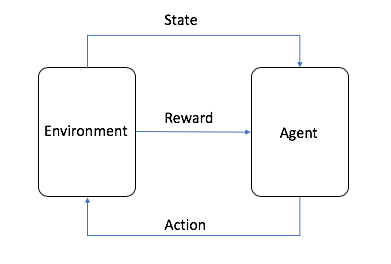
\includegraphics[width=140mm, height=140mm]{./agent_enviroment}
\caption{Herní cyklus}
\label{obr03:Nhust}
\end{figure}
